\section{Progress}

\begin{frame}
\frametitle{Initial Prototype}
\begin{figure}
\centering
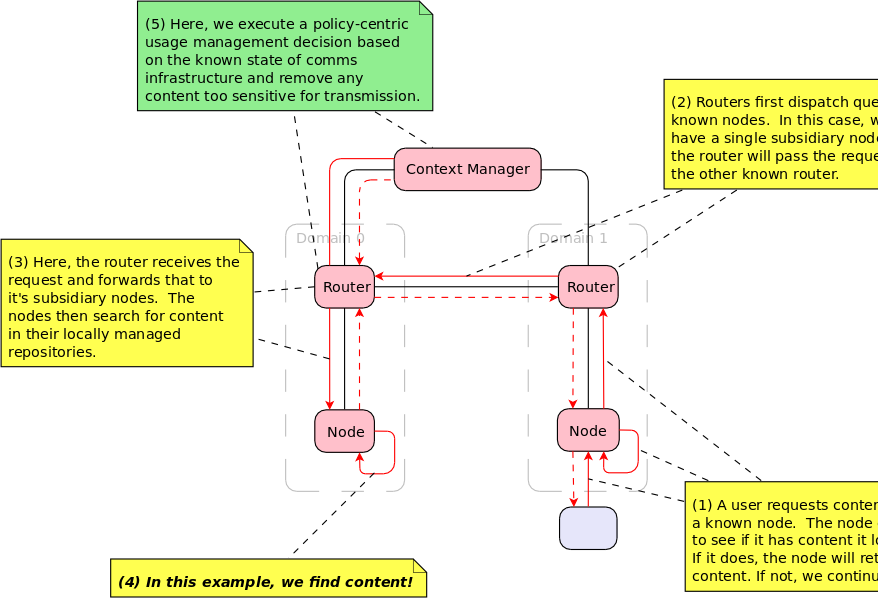
\includegraphics[width=4in]{cross-domain-prototype}
\label{fig:implementation:prototype}
\end{figure}
\end{frame}

\begin{frame}
\frametitle{Current Work}
We're currently extending the local simulation to a distributed content system.  The environment we're using consists of roughly 40 nodes distributed over Rackspace (using Rackspace Servers), Amazon (using EC2), and our local Eucalyptus installation.  We will use Heroku as well (We're deliberately building networks over providers and mixing IAAS and PAAS).
\newline
\pause
\begin{itemize}
\item \textit{Ruby} --- We use Ruby and the Ruby runtime as our base runtime engine.  We use associated tools like RVM, Gem, and Bundler to manage our projects.
\pause
\item \textit{Sinatra} --- Sintara is a simple but powerful HTTP engine.
\pause
\item \textit{Capistrano} --- Capistrano simplifies deployment of software on large numbers of nodes.
\pause
\item \textit{YAML} --- YAML is a simple data serialization language.
\end{itemize}
\end{frame}

\begin{frame}[c]
\frametitle{Future Work}
We are in the process of configuring infrastructure to begin work with Openflow-enabled hardware.  We will use Ruby and ruby tools in this environment as well, with the addition of Trema, a Ruby and C based environment for building Openflow controllers.
Openflow and Software Defined Networking.
\end{frame}